\section{Week 1}

\subsection{Introduction to LLM and RAG}
\footnote{\href{https://www.youtube.com/watch?v=Q75JgLEXMsM&list=PL3MmuxUbc_hIB4fSqLy_0AfTjVLpgjV3R&index=1}{Lecture 1}}A language model is a model which predicts the next word based on the words which you have typed so far. A \textbf{Large Language model} also does the same thing,
but has a lot more parameters (billions).
The input to the LLMS (text/image/video etc.) is called prompt.\\
\textbf{RAG} stands for Retrieval Augmented Generation. Retrieval means search, so a RAG system uses search to augment the generation (make it better) of the text.

\begin{figure}[h]
    \centering
    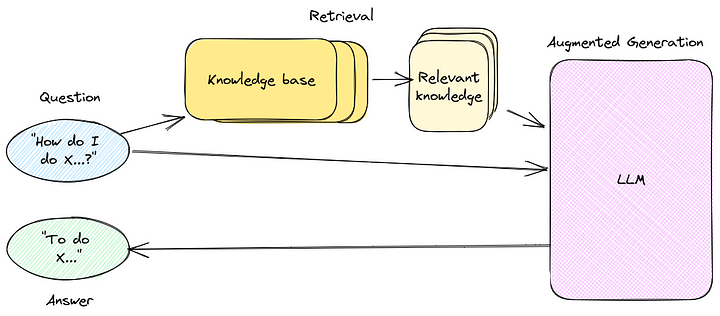
\includegraphics[width=0.6\textwidth]{media/rag_system.png}
    \caption{RAG system overview}
    \label{fig:mesh1}
\end{figure}

\subsection{Preparing the Environment}
\begin{lstlisting}
python3 -m venv myenv
source myenv/bin/activate\end{lstlisting}
\footnote{\href{https://www.youtube.com/watch?v=ozCpmkbJNJE&list=PL3MmuxUbc_hIB4fSqLy_0AfTjVLpgjV3R&index=2}{Lecture 2}}
Commands \verb|which python3| and \verb|python3 -V| can be used to check source and version of python.
\begin{lstlisting}
pip install tqdm openai elasticsearch scikit-learn pandas
pip freeze > requirements.txt\end{lstlisting}
OpenAI api key can be obtained from \href{https://platform.openai.com/api-keys}{here}.
\begin{lstlisting}
load_dotenv()
openai_key = os.getenv('OPENAI_KEY')
###
client.chat.completions.create(
    model='gpt-3.5-turbo',
    messages=[
       {
        "role": "user",
        "content": "What is up?"
       }
    ]
)\end{lstlisting}
\begin{itemize}
    \item messages is what we write to the client
\end{itemize}
\subsection{Retrieval}
xxx
\subsection{Generation with OpenAI}

\subsubsection{OpenAI API Alternatives}

\subsection{Cleaned RAG flow}

\subsection{Searching with ElasticSearch}